
\begin{table*}
\centering
{\small
    \begin{tabular}{|l|l|c|c|c|c|c|c|c|}
    \hline
	\multirow{2}{*}{~}			& \multirow{2}{*}{Approach}		& \multirow{2}{*}{\parbox{2.2cm}{Sleep Interval (seconds)}}	
																						& \multicolumn{3}{c|}{Average Power (mW)}		& \multicolumn{3}{c|}{Recall} 													\\ \cline{4-9}
								&								&						& Steps		& Headbutts	& Transitions	& Steps					& Headbutts					& Transitions 				\\ \hline
	\multirow{14}{*}{\parbox{1.2cm}{Group 1 90\% idle}}	& \multicolumn{2}{l|}{Always Awake}						& \multicolumn{3}{c|}{323}				& \multirow{6}{*}{98\%}	& \multirow{6}{*}{100\%}	& \multirow{6}{*}{100\%}	\\ \cline{2-6}
								& \multirow{5}{*}{Batching}		& 2						& \multicolumn{3}{c|}{350}				&						&							&							\\ \cline{3-6}
								& 								& 5						& \multicolumn{3}{c|}{186}				&						&							&							\\ \cline{3-6}
								& 								& 10					& \multicolumn{3}{c|}{115}				&						&							&							\\ \cline{3-6}
								& 								& 20					& \multicolumn{3}{c|}{80.1}				&						&							&							\\ \cline{3-6}
								& 								& 30					& \multicolumn{3}{c|}{68.3}				&						&							&							\\ \cline{2-9}
								& \multirow{5}{*}{Duty Cycling}	& 2						& \multicolumn{3}{c|}{339}				& 94\%					& 57\%						& 97\%						\\ \cline{3-9}
								& 								& 5						& \multicolumn{3}{c|}{217}				& 82\%					& 14\%						& 47\%						\\ \cline{3-9}
								& 								& 10					& \multicolumn{3}{c|}{140}				& 63\%					& 29\%						& 28\%						\\ \cline{3-9}
								& 								& 20					& \multicolumn{3}{c|}{86.3}				& 48\%					& 14\%						& 32\%						\\ \cline{3-9}
								& 								& 30					& \multicolumn{3}{c|}{63.1}				& 31\%					& 7\%						& 12\%						\\ \cline{2-9}
								& \multicolumn{2}{l|}{Predifined Activity}				& \multicolumn{3}{c|}{48.3}				& \multirow{3}{*}{98\%}	& 36\%						& 87\%						\\ \cline{2-6}\cline{8-9}
								& \multicolumn{2}{l|}{Smartsensor}						& 48.3		& 60.3		& 18.6			& 						& \multirow{2}{*}{100\%}	& \multirow{2}{*}{100\%}	\\ \cline{2-6}
								& \multicolumn{2}{l|}{Oracle}							& 41.5		& 59.6		& 16.4			& 						& 							& 							\\ \hline \hline
								
	\multirow{14}{*}{\parbox{1.2cm}{Group 2 50\% idle}}	& \multicolumn{2}{l|}{Always Awake}						& \multicolumn{3}{c|}{323}				& \multirow{6}{*}{99\%}	& \multirow{6}{*}{100\%}	& \multirow{6}{*}{100\%}	\\ \cline{2-6}
								& \multirow{5}{*}{Batching}		& 2						& \multicolumn{3}{c|}{350}				&						&							&							\\ \cline{3-6}
								& 								& 5						& \multicolumn{3}{c|}{186}				&						&							&							\\ \cline{3-6}
								& 								& 10					& \multicolumn{3}{c|}{115}				&						&							&							\\ \cline{3-6}
								& 								& 20					& \multicolumn{3}{c|}{80.1}				&						&							&							\\ \cline{3-6}
								& 								& 30					& \multicolumn{3}{c|}{68.3}				&						&							&							\\ \cline{2-9}
								& \multirow{5}{*}{Duty Cycling}	& 2						& \multicolumn{3}{c|}{334}				& 92\%					& 74\%						& 90\%						\\ \cline{3-9}
								& 								& 5						& \multicolumn{3}{c|}{243}				& 79\%					& 31\%						& 53\%						\\ \cline{3-9}
								& 								& 10					& \multicolumn{3}{c|}{176}				& 65\%					& 20\%						& 36\%						\\ \cline{3-9}
								& 								& 20					& \multicolumn{3}{c|}{106}				& 33\%					& 5\%						& 10\%						\\ \cline{3-9}
								& 								& 30					& \multicolumn{3}{c|}{80}				& 25\%					& 11\%						& 12\%						\\ \cline{2-9}
								& \multicolumn{2}{l|}{Predifined Activity}				& \multicolumn{3}{c|}{188}				& \multirow{3}{*}{99\%}	& 13\%						& 73\%						\\ \cline{2-6}\cline{8-9}
								& \multicolumn{2}{l|}{Smartsensor}						& 188		& 65.1		& 43.3			& 						& \multirow{2}{*}{100\%}	& \multirow{2}{*}{100\%}	\\ \cline{2-6}
								& \multicolumn{2}{l|}{Oracle}							& 153		& 62.3		& 29.5			& 						& 							& 							\\ \hline \hline

	\multirow{14}{*}{\parbox{1.2cm}{Group 3 10\% idle}}	& \multicolumn{2}{l|}{Always Awake}						& \multicolumn{3}{c|}{323}				& \multirow{6}{*}{97\%}	& \multirow{6}{*}{100\%}	& \multirow{6}{*}{100\%}	\\ \cline{2-6}
								& \multirow{5}{*}{Batching}		& 2						& \multicolumn{3}{c|}{350}				&						&							&							\\ \cline{3-6}
								& 								& 5						& \multicolumn{3}{c|}{186}				&						&							&							\\ \cline{3-6}
								& 								& 10					& \multicolumn{3}{c|}{115}				&						&							&							\\ \cline{3-6}
								& 								& 20					& \multicolumn{3}{c|}{80.1}				&						&							&							\\ \cline{3-6}
								& 								& 30					& \multicolumn{3}{c|}{68.3}				&						&							&							\\ \cline{2-9}
								& \multirow{5}{*}{Duty Cycling}	& 2						& \multicolumn{3}{c|}{332}				& 89\%					& 47\%						& 89\%						\\ \cline{3-9}
								& 								& 5						& \multicolumn{3}{c|}{257}				& 76\%					& 28\%						& 26\%						\\ \cline{3-9}
								& 								& 10					& \multicolumn{3}{c|}{198}				& 64\%					& 27\%						& 25\%						\\ \cline{3-9}
								& 								& 20					& \multicolumn{3}{c|}{133}				& 42\%					& 19\%						& 19\%						\\ \cline{3-9}
								& 								& 30					& \multicolumn{3}{c|}{99.1}				& 30\%					& 9\%						& 14\%						\\ \cline{2-9}
								& \multicolumn{2}{l|}{Predifined Activity}				& \multicolumn{3}{c|}{321}				& \multirow{3}{*}{97\%}	& 95\%						& 86\%						\\ \cline{2-6}\cline{8-9}
								& \multicolumn{2}{l|}{Smartsensor}						& 321		& 65.7		& 51.7			& 						& \multirow{2}{*}{100\%}	& \multirow{2}{*}{100\%}	\\ \cline{2-6}
								& \multicolumn{2}{l|}{Oracle}							& 266		& 62.9		& 34.9			& 						& 							& 							\\ \hline
    \end{tabular}
}
	\caption{Event recall and average power for synthetic traces.}
	\label{table:summaryRecallPower}
\end{table*}


\section{Results}
\label{sec:results}

In this section we first present the result of experiments conducted
on synthetic traces collected with our robotic platform.  We then
present preliminary results from on a small number of traces collected
from human subjects.  Finally, we reflect on the effects that an-board
Smartsensor implementation would have on our results.

\subsection{Synthetic Traces}

We experimented with our synthetic traces to answer the following questions:

\begin{enumerate}
\setlength{\itemsep}{-3pt}  

\item What are the benefits of Smartsensor over Duty Cycling and
  Batching?

\item Can Predefined Activity support a broad set of applications?

\item How much additional benefit can be obtained from fully
  programmable wake-up conditions?

\item Are multiple different filters required, and how important it is
  to let the application configure the filter parameters and
  thresholds?

\end{enumerate}

\subsubsection{Smartsensor vs. Duty Cycling and Batching}

Table~\ref{table:summaryRecallPower} presents the results of replaying
the traces collected from the robot for the sensing approaches
described in the previous section.  For each application, the table
presents average power consumption and activity recall.  Results are
averages over all the runs of the same group.  The results for the
Always Awake approach provide a base line for comparison.  While the
point of this work was not to create perfect activity detectors, the
Always Awake implementations achieve close to perfect recall.  All
sensing approaches achieved similar average precision (Headbutts:
89\%, Transitions: 91\%, Walking: 0.93\%), and we therefore do not
include these numbers in the table.

As expected, Duty Cycling performs poorly.  Short sleep intervals
actually result in an increase in power consumption due to frequent
transitioning between awake and asleep states.  Longer sleep interval
are more effective at saving energy, but they do so by sacrificing
recall.  For example, a sleep interval of 10 seconds reduces the
Headbutts and Transittions recall bellow 30\%.

Batching matches the recall of Always Awake, but requires long
batching intervals to achieve large energy savings.  Therefore, this
approach may not be appropriate for applications with real time
constrains.  For example, the user of a gesture recognition
application~\cite{liu2009uwave,schlomer2008gesture} would not be
satisfied if the application detects the performed gesture after a
delay of more than a couple of seconds.  We anticipate that in
practice realistic batching intervals are in the order of a few
seconds.  We therefore conclude, that batching will result in
significant energy waste for applications interested in low frequency
events (e.g., gesture recognition, fall detection).

Smartsensor achieved the lowest power consumption in every scenario
other than step detection in group 3. All these scenarios are similar
in that the event of interest occurs infrequently (less than 15\% of
the time). Walking represents about 63\% of the courses in group 3.
For this scenario, only the batching approach achieved better power
savings.


\subsubsection{Smartsensor vs Predefined Activity}

Predefined Activity performs very well for step detection (as
expected), but results in either poor recall or low energy savings for
the other two applications.  We conclude that hardware support for
predefined activity detection may work well for a small set of
application, but is inefficient for most other applications. As such,
developers should be able to configure the wake-up conditions based on
the needs of their applications.

\subsubsection{Smartsensor vs. Oracle}

By comparing the performance of the Smartsensor approach to Oracle we
observe that for most usage scenarios, the Smartsensor approach
achieves over 95\% of the available power saving.  We conclude that
there is little additional benefit that could be obtained by providing
application developer with ability to create fully programmable
wake-up conditions.


\begin{table*}[t]
\centering
{\small
    \begin{tabular}{|l|l|c|c|c|c|c|}
	\hline
    \multirow{2}{*}{Sensor Data Filter}    	& \multicolumn{3}{c|}{Power Consumption (mW)} \\ \cline{2-4}
							& Steps	& Headbutts	& Transitions 	\\ \hline
    Null     				& 191		& 186		& 67.8 			\\ \hline
	EMA   				& {\bf 188}		& 228		& {\bf 43.3} 			\\ \hline
	FFT 				& 217		& {\bf 65.1} 		& 88.7 			\\ \hline
	
    \end{tabular}
}
	\caption{Average power for Group 2 runs with different filters.}
	\label{table:WUCfilters}
\end{table*}

\subsubsection{Filter Selection and Configuration}

Table~\ref{table:WUCfilters} shows the energy saving using three
different filters for each application.  For each condition, the
filter uses the parameters and thresholds that maximize energy saving
while matching the application recall of Always Awake.  The condition
that achieves the best power saving is highlighted.  The results show
that different data filters are optimal for different applications.
Even in cases where the same filter type is optimal, the configuration
parameters for the filter and the wake-up thresholds different
significantly.  

Figure\ref{fig:wucHeadbuttFFTRecallPowerGroup3} uses the Heabbutt
application to ilustrate the sensitivity of application recall and
power to threshold selection.  A threshold that is too strict causes a
significant drop-off in the achieved recall.  However, choosing a
threshold that is too lenient results in additional power consumption
without any extra benefit to recall because of unnecessary wake-ups.

\begin{figure}[h]
	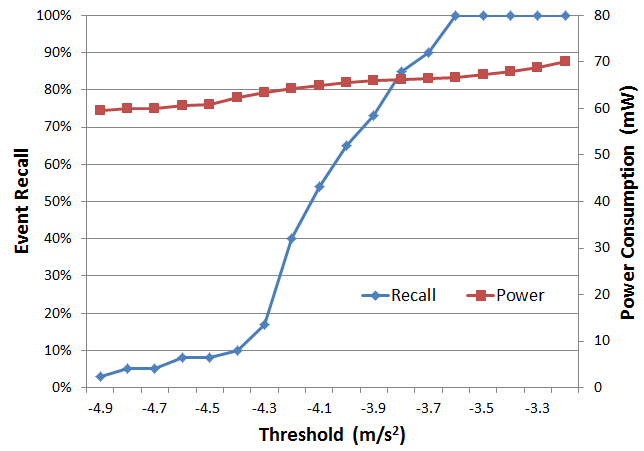
\includegraphics[width=3.1in]{wuc_hb_fft_group3.png}
	\caption{Threshold sensitivity for Headbutts application}
    \label{fig:wucHeadbuttFFTRecallPowerGroup3}
\end{figure}

We conclude that in order to optimize performance, applicaitons should
be allowed both select an optimal filter as well as configure its
parameters and thresholds.

\subsection{Human Traces}

Table~\ref{table:macrobenchmarks} shows the results from running the
step detector application on traces collected from three human
subjects.  Since these traces are not annotated with ground thruth, we
use the steps detected by the Always Awake as the baseline for
determining recall.

Remarkably the results from these experiments show very similar
benefits to the synthetic experiments for runs with low and medium
levels of activity.  For example, the energy saving for the
Smartsensor approach come within X\% of Oracle.


\begin{table*}[t]
\centering
{\small
    \begin{tabular}{|l|c|c|c|c|c|c|}
    \hline
	\multirow{2}{*}{Approach}		& \multirow{2}{*}{\parbox{2.2cm}{Sleep Interval (seconds)}}
												& \multicolumn{3}{c|}{\parbox{3.2cm}{Power (mW)}}
																								& \multirow{2}{*}{\parbox{1.5cm}{Average Recall}} \\ \cline{3-5}
									&			& Trace 1		& Trace 2		& Trace 3 		& 							\\ 
									&			& 37\% walking	& 22\% walking		& 20\% walking		& \\ \hline
	Always Awake					& 			& \multicolumn{3}{c|}{323} 						& 100\% \\ \hline
	\multirow{5}{*}{Duty Cycling}	& 2			& 329			& 330			& 330			& 97\%	\\ \cline{2-6}
									& 5			& 272			& 260			& 261			& 92\%	\\ \cline{2-6}
									& 10		& 220			& 195			& 198			& 82\%	\\ \cline{2-6}
									& 20		& 172			& 131			& 134			& 66\%	\\ \cline{2-6}
									& 30		& 148			& 104			& 106			& 57\%	\\ \hline
	\multirow{5}{*}{Batching}		& 2			& \multicolumn{3}{c|}{350} 						& 100\% \\ \cline{2-6}
									& 5			& \multicolumn{3}{c|}{186} 						& 100\% \\ \cline{2-6}
	 								& 10		& \multicolumn{3}{c|}{115} 						& 100\% \\ \cline{2-6}
	 								& 20		& \multicolumn{3}{c|}{80.1} 					& 100\% \\ \cline{2-6}
	 								& 30		& \multicolumn{3}{c|}{68.3} 					& 100\% \\ \hline
	Smartsensor				&			& 136			& 77.9			& 72.6			& 100\% \\ \hline
	Oracle				&			& 117.8			& 65.8			& 62.3			& 100\% \\ \hline



    \end{tabular}
}
	\caption{Event recall and power consumption for human traces.}
	\label{table:macrobenchmarks}
\end{table*}

\subsection{Discussion}

{\em TODO An integrated implemetation is likely to be more power
  efficient. How does this affect these results?}
